\documentclass{article}

\usepackage{amsmath, mathtools, amsthm, booktabs, float, hyperref}

\usepackage{graphicx}
\graphicspath{ {../images/tps/} }

\title{Centralina di irrigazione}
\author{Lena Giovanni Leonardo}
\date{\today}

\begin{document}
    \maketitle

    \section{Criteri}

    \begin{enumerate}
        \item Ci deve essere un controllo di accensione generale, (INGRESSO ON/OFF)
        \item La pompa può essere azionata solo se il livello del serbatoio è superiore ad una soglia indicata da un sensore di livello (INGRESSO LIVELLO)
        \item L’irrigazione può essere effettuata solo se siamo di notte, possiamo usare una fotocellula oppure un timer (INGRESSO ABILITAZIONE)
        \item ovviamente si irrigherà soltanto se un sensore di umidità posto nel terreno indicherà se il terreno è asciutto e non umido (INGRESSO UMIDITA’)
        \item Si deve prevedere anche un ingresso che viene attivato se la pompa si trova in avaria (INGRESSO PROTEZIONE), con eventuale accensione di un’uscita (USCITA AVARIA).
    \end{enumerate}

    \section{Lista ingressi}

    \begin{enumerate}
        \item Generale (attivo alto)
        \item Livello OK (attivo alto)
        \item Abilitazione notte (attivo alto)
        \item Umidità OK (attivo alto)
        \item Protezione OK (attivo alto)
    \end{enumerate}

    \section{Lista uscite}

    \begin{enumerate}
        \item Pompa (attivo alto)
        \item Avaria (attivo alto)
    \end{enumerate}

    \section{Layout impianto}

    \begin{center}
        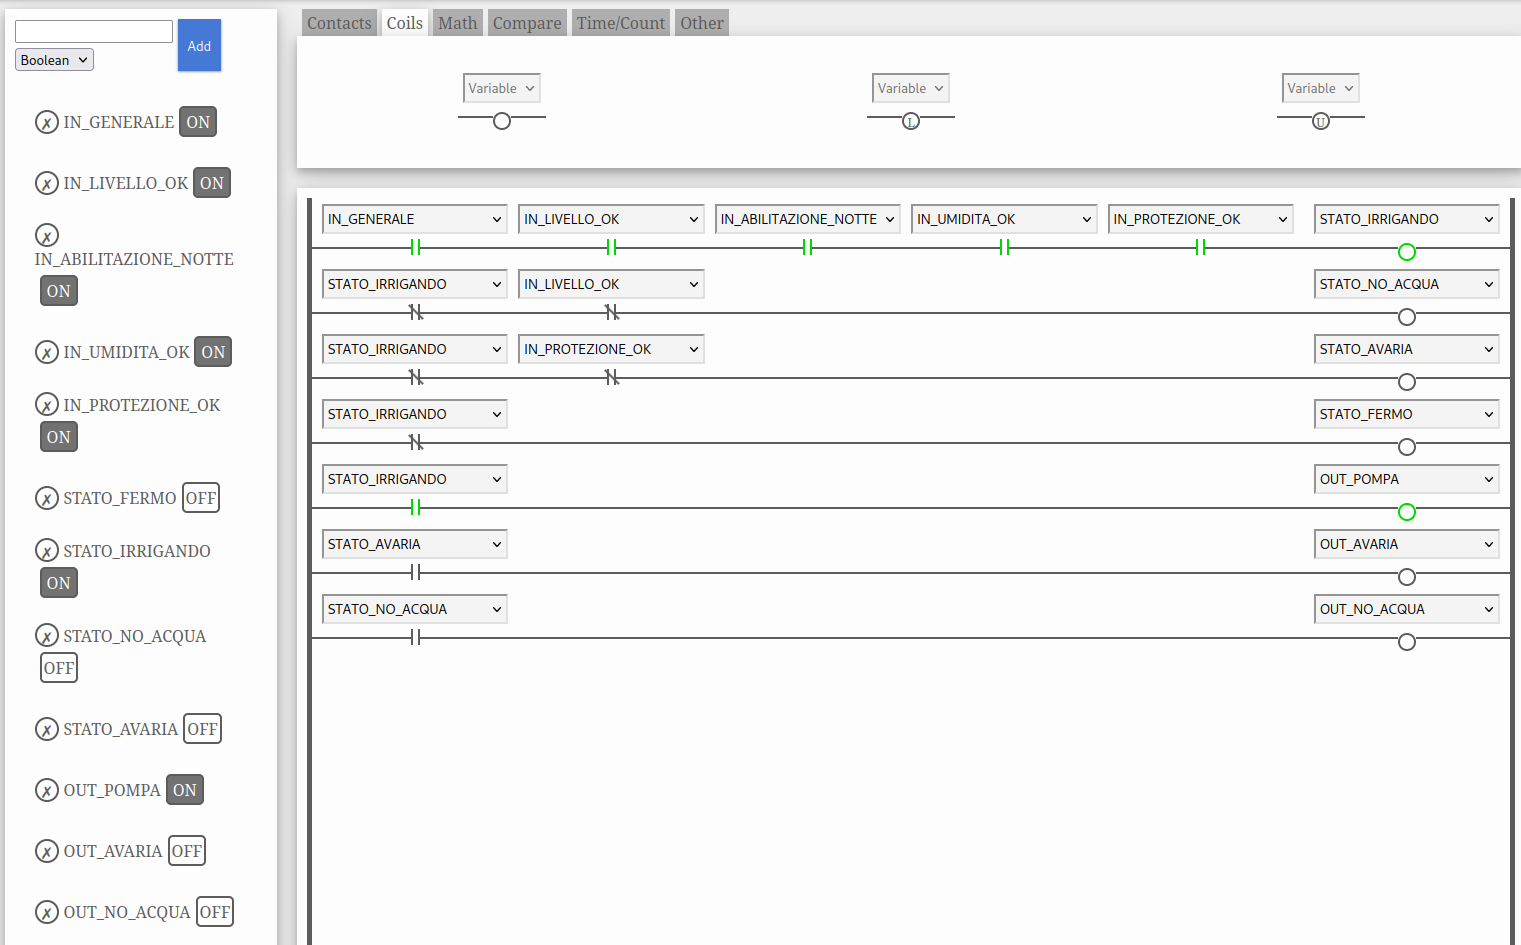
\includegraphics[width=\textwidth]{esercizio_irrigazione.png}
    \end{center}

    \section{Tabella di verità (uscita pompa)}

    \begin{table}[H]
    \centering
    \resizebox{\textwidth}{!}{
    \begin{tabular}{|l|l|l|l|l|l|}
    \hline
    Generale & Livello & Abilitazione & Umidità & Protezione & Pompa \\ \hline
    1        & 1       & 1            & 1       & 1          & 1     \\ \hline
    0        & *       & *            & *       & *          & 0     \\ \hline
    *        & 0       & *            & *       & *          & 0     \\ \hline
    *        & *       & 0            & *       & *          & 0     \\ \hline
    *        & *       & *            & 0       & *          & 0     \\ \hline
    *        & *       & *            & *       & 0          & 0     \\ \hline
    \end{tabular}
    }
    \end{table}

    (* indica qualsiasi valore)

    \section{Tabella di verità (uscita avaria)}

    \begin{table}[H]
    \centering
    \resizebox{\textwidth}{!}{
    \begin{tabular}{|l|l|l|l|l|l|}
    \hline
    Generale & Livello & Abilitazione & Umidità & Protezione & Avaria \\ \hline
    *        & *       & *            & *       & 1          & 0      \\ \hline
    *        & *       & *            & *       & 0          & 1      \\ \hline
    \end{tabular}
    }
    \end{table}

    (* indica qualsiasi valore)

    \section{Versione interattiva}
    \href{https://www.plcfiddle.com/fiddles/9cbc64a1-7816-46ec-b24b-27cd1a673e36http://www.overleaf.com}{https://www.plcfiddle.com/fiddles/9cbc64a1-7816-46ec-b24b-27cd1a673e36}

\end{document}
